\chapter{Создание макета системы управления микроклиматом теплицы}

\section{Условное графическое представление макета с разбиением на функциональные и структурные блоки}

Функционально макет можно разделить на ряд блоков, каждый из которых будет представлять собой подсистему. Функциональная схема данного макета представлена на рис.~\ref{fig:func_schem}.

Структурная схема макета дает лучшее представление о последовательности взаимодействия функциональных частей макета и представлена на рис.~\ref{fig:struct_schem}.

\begin{figure}[H]
    \centering
    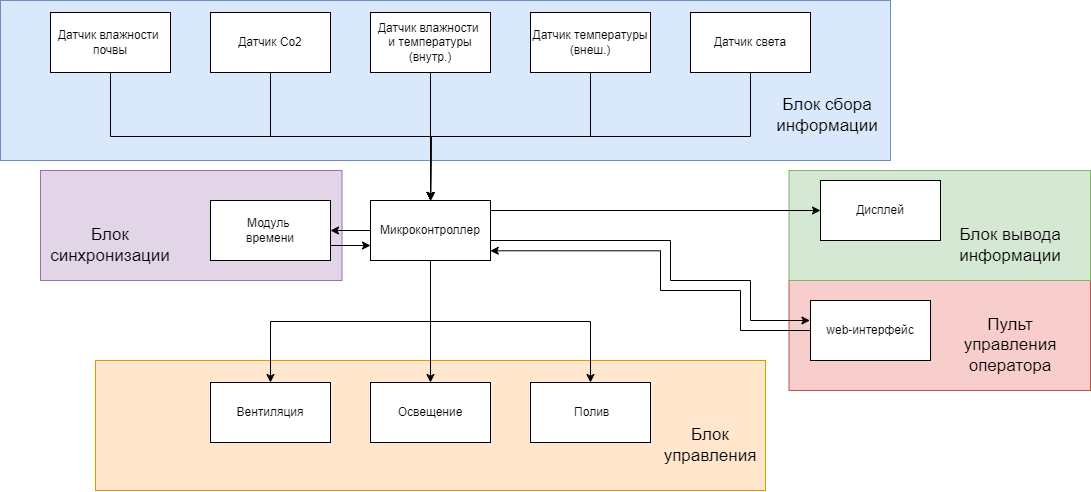
\includegraphics[scale=0.4]{images/struct_schem.png}
    \caption{Структурная схема макета умной теплицы}
    \label{fig:struct_schem}
\end{figure}

% TODO: Желательно при описании составляющих модулей описывать их в виде таблицы
\subsection{Модуль управления макетом}

Модуль управления макетом состоит из микроконтроллера ESP32.%Его краткие технические характеристики приведены в таблице:
% \begin{table}[]
%     \centering
%     \begin{tabular}{c|c}
%          &  \\
%          & 
%     \end{tabular}
%     \caption{Caption}
%     \label{tab:my_label}
% \end{table}

%Убрать обычный текст

Управляющий контроллер ESP32 --- это микроконтроллер, разработанный компанией Espressif Systems. Он используется в широком спектре устройств, включая умные дома, умные гаджеты, Интернет вещей (IoT) и т.д. Одной из его главных особенностей является интеграция беспроводных технологий, таких как Wi-Fi и Bluetooth;

\begin{figure}[H]
    \centering
    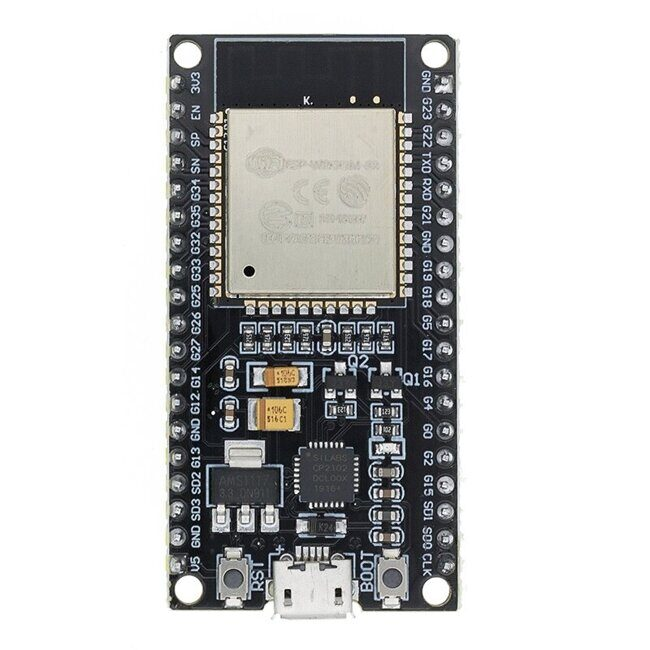
\includegraphics[scale=0.45]{images/esp.jpg}
    \caption{Управляющий контроллер ESP-32(отладочная плата)}
    \label{fig:esp}
\end{figure}

\subsection{Модуль измерения параметров окружающей среды}

Данная Модуль представляет из себя набор различных датчиков для измерения параметров окружающей среды, среди которых:

\begin{enumerate}
    \item емкостной датчик влажности почвы. Емкостной датчик влажности почвы --- это электронный датчик, который использует изменение емкости для измерения влажности почвы. Датчик состоит из двух электродов, которые помещаются в почву. В зависимости от влажности почвы, емкость между электродами меняется, что затем используется для определения уровня влажности;

    \begin{figure}[H]
        \centering
        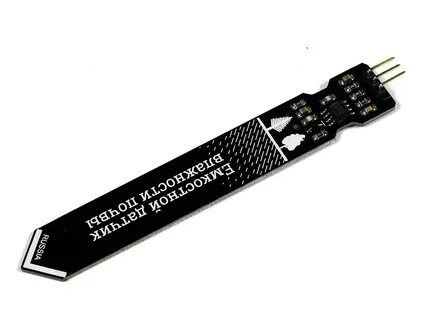
\includegraphics[scale=0.6]{images/wet.jpg}
        \caption{Емкостной датчик влажности почвы}
        \label{fig:wet}
    \end{figure}
    %Его краткие технические характеристики приведены в таблице:
    % \begin{table}[]
    %     \centering
    %     \begin{tabular}{c|c}
    %          &  \\
    %          & 
    %     \end{tabular}
    %     \caption{Caption}
    %     \label{tab:my_label}
    % \end{table}
    
    %Убрать обычный текст

    \item датчик углекислого газа MQ-7. MQ-7 --- это электрохимический датчик углекислого газа, используемый для измерения концентрации CO2 в воздухе. Он использует токсичный газовый сенсор, который реагирует на уровень CO2 в воздухе и преобразует его в сигнал напряжения. Этот сигнал может быть интерпретирован микроконтроллером для определения уровня CO2 в окружающей среде;

    \begin{figure}[H]
        \centering
        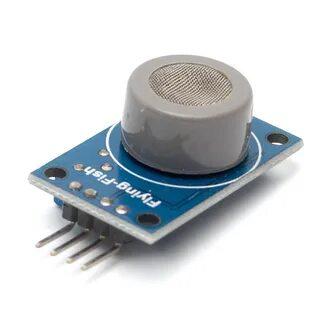
\includegraphics[scale=0.6]{images/mq7.jpg}
        \caption{Датчик Co2 MQ-7}
        \label{fig:mq7}
    \end{figure}
    %Его краткие технические характеристики приведены в таблице:
    % \begin{table}[]
    %     \centering
    %     \begin{tabular}{c|c}
    %          &  \\
    %          & 
    %     \end{tabular}
    %     \caption{Caption}
    %     \label{tab:my_label}
    % \end{table}
    
    %Убрать обычный текст
    
    \item датчик влажности воздуха и температуры DHT11. DHT11 --- это цифровой датчик влажности воздуха и температуры для использования с микроконтроллерами. Он имеет простой интерфейс и может быть легко подключен с помощью всего трех выводов. DHT11 использует однопроводную шину для передачи данных и измеряет температуру в диапазоне от 0 до 50 градусов Цельсия и относительную влажность в диапазоне от 20\% до 90\%. Данные от датчика могут быть легко считаны и обработаны с помощью Arduino и других платформ;

    \begin{figure}[H]
        \centering
        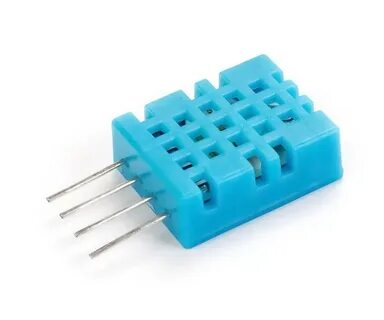
\includegraphics[scale=0.6]{images/dht11.jpg}
        \caption{Датчик влажности и температуры DHT11}
        \label{fig:dht11}
    \end{figure}
    %Его краткие технические характеристики приведены в таблице:
    % \begin{table}[]
    %     \centering
    %     \begin{tabular}{c|c}
    %          &  \\
    %          & 
    %     \end{tabular}
    %     \caption{Caption}
    %     \label{tab:my_label}
    % \end{table}
    
    %Убрать обычный текст
    
    \item датчик освещенности BH1750. Датчик освещенности BH1750FVI --- это цифровой датчик, используемый для измерения уровня освещенности в окружающей среде. Он работает на основе принципа фотодиодного преобразования и имеет широкий диапазон измерений --- от 1 до 65535 люксов. Датчик может быть подключен к микроконтроллеру через интерфейс I2C, что делает его легко интегрируемым в проекты с использованием платформы Arduino или других микроконтроллеров;

    \begin{figure}[H]
        \centering
        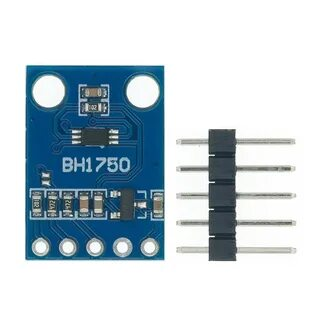
\includegraphics[scale=0.6]{images/bh1750.jpg}
        \caption{Датчик освещенности BH1750}
        \label{fig:bh1750}
    \end{figure}
    %Его краткие технические характеристики приведены в таблице:
    % \begin{table}[]
    %     \centering
    %     \begin{tabular}{c|c}
    %          &  \\
    %          & 
    %     \end{tabular}
    %     \caption{Caption}
    %     \label{tab:my_label}
    % \end{table}
    
    %Убрать обычный текст
    
    \item датчик температуры (внешний) DS18B20. DS18B20 --- это цифровой датчик температуры, который может измерять температуру в диапазоне от -55 до +125 градусов Цельсия. Он имеет компактный размер и использует одну цифровую линию для передачи данных, что делает его удобным для использования с микроконтроллерами, такими как Arduino. DS18B20 также может работать в режиме питания от 3,0 до 5,5 В, что позволяет его использовать с различными источниками питания;

    \begin{figure}[H]
        \centering
        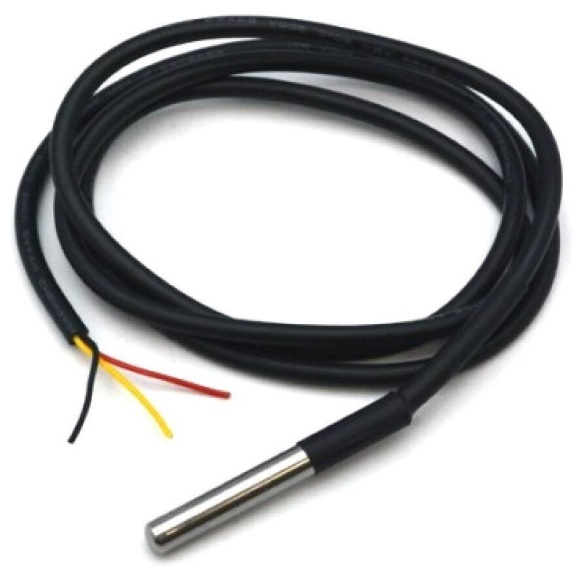
\includegraphics[scale=0.8]{images/temperature.jpg}
        \caption{Датчик температуры DS18B20}
        \label{fig:temp}
    \end{figure}
    %Его краткие технические характеристики приведены в таблице:
    % \begin{table}[]
    %     \centering
    %     \begin{tabular}{c|c}
    %          &  \\
    %          & 
    %     \end{tabular}
    %     \caption{Caption}
    %     \label{tab:my_label}
    % \end{table}
    
    %Убрать обычный текст
\end{enumerate}

\subsection{Модуль отображения параметров среды}

В качестве подсистемы отображения параметров окружающей среды выступает LCD-дисплей и модуль часов реального времени для точной привязки показаний к текущему времени.

LCD-дисплей 1602 --- это тип жидкокристаллического дисплея, который имеет 2 строки и 16 символов в каждой строке. Он широко используется в различных электронных проектах, таких как умные дома, термостаты, часы и другие устройства, которые требуют вывода небольшого объема информации на экран. Дисплей 1602 управляется с помощью контроллера HD44780, который поддерживает стандартный протокол интерфейса параллельной шины для связи с микроконтроллером;

\begin{figure}[H]
    \centering
    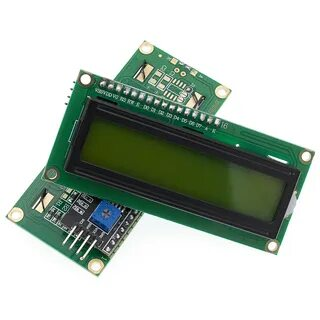
\includegraphics{images/lcd.jpg}
    \caption{LCD дисплей 1602}
    \label{fig:lcd}
\end{figure}
%Его краткие технические характеристики приведены в таблице:
% \begin{table}[]
%     \centering
%     \begin{tabular}{c|c}
%          &  \\
%          & 
%     \end{tabular}
%     \caption{Caption}
%     \label{tab:my_label}
% \end{table}

%Убрать обычный текст

Модуль часов реального времени DS1307 --- это устройство, которое можно подключить к плате, чтобы обеспечить точное хранение и отслеживание времени. Он использует кварцевый резонатор для генерации точной временной метки, которая может сохраняться даже при отключении питания. Модуль имеет интерфейс I2C для связи с микроконтроллером и может быть программирован для установки текущего времени и даты. DS1307 также может использоваться для контроля временных интервалов и для триггеров на основе времени. Он питается от батарейки, что обеспечивает длительный срок службы без перезагрузки или сброса времени;

\begin{figure}[H]
    \centering
    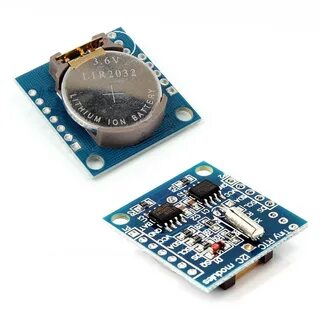
\includegraphics[scale=0.6]{images/ds1307.jpg}
    \caption{Модуль часов реального времени}
    \label{fig:ds1307}
\end{figure}

%Его краткие технические характеристики приведены в таблице:
% \begin{table}[]
%     \centering
%     \begin{tabular}{c|c}
%          &  \\
%          & 
%     \end{tabular}
%     \caption{Caption}
%     \label{tab:my_label}
% \end{table}

%Убрать обычный текст

\subsection{Модуль элементов поддержания параметров теплицы}

Для поддержания необходимых параметров окружающей среды в макете используются:

\begin{enumerate}
    \item вентиляция (куллеры);
    %Его краткие технические характеристики приведены в таблице:
    % \begin{table}[]
    %     \centering
    %     \begin{tabular}{c|c}
    %          &  \\
    %          & 
    %     \end{tabular}
    %     \caption{Caption}
    %     \label{tab:my_label}
    % \end{table}
    
    %Убрать обычный текст
    
    \item система полива (помпа) AD20P-1230C. Помпа AD20P-1230C – это компактная насосная станция, которая используется для перекачки воды и других жидкостей. Она может применяться в различных областях, включая бытовую и промышленную сферы. Помпа имеет компактные размеры и небольшой вес, что облегчает установку и транспортировку, низкий уровень шума работы, высокую производительность и эффективность;

    \begin{figure}[H]
        \centering
        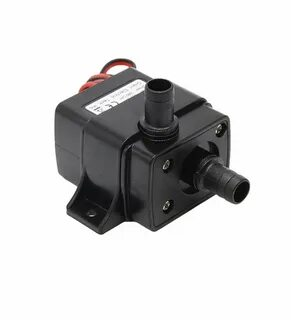
\includegraphics[scale=0.6]{images/pump.jpg}
        \caption{Помпа AD20P-1230C}
        \label{fig:pump}
    \end{figure}
    %Его краткие технические характеристики приведены в таблице:
    % \begin{table}[]
    %     \centering
    %     \begin{tabular}{c|c}
    %          &  \\
    %          & 
    %     \end{tabular}
    %     \caption{Caption}
    %     \label{tab:my_label}
    % \end{table}
    
    %Убрать обычный текст
    
    \item система освещения (Светодиодная лента) IP65. Фитолента IP65 –-- это специальная светодиодная лента, разработанная для обеспечения растений в теплицах, оранжереях и других закрытых помещениях необходимым количеством света для нормального роста и развития.

    \begin{figure}[H]
        \centering
        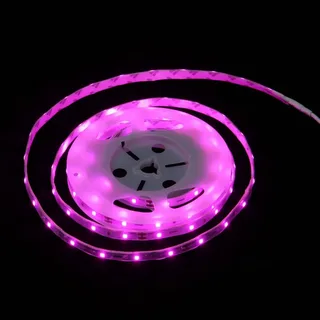
\includegraphics[scale=0.8]{images/ip65.png}
        \caption{Фитолента IP65}
        \label{fig:ip65}
    \end{figure}
    
    Фитолента IP65 обладают следующими характеристиками:
    
    \begin{enumerate}
        \item устойчивость к влаге и пыли благодаря защитному покрытию IP65;
        \item высокая яркость светодиодов для обеспечения необходимого уровня освещения растений;
        \item низкое потребление электроэнергии;
        \item возможность регулировки яркости и цветовой температуры;
        \item гибкость и легкость монтажа на любой поверхности;
        \item долгий срок службы и надежность работы.
    \end{enumerate}
\end{enumerate}
%Его краткие технические характеристики приведены в таблице:
% \begin{table}[]
%     \centering
%     \begin{tabular}{c|c}
%          &  \\
%          & 
%     \end{tabular}
%     \caption{Caption}
%     \label{tab:my_label}
% \end{table}

%Убрать обычный текст

Схема соединений для данного макета иллюстрирует связи входных и выходных элементов и устройств и представлена на рис.~\ref{fig:connection_schem} в Приложении А.

\section{Основные технические требования к макету}

Список требований, которые предъявляются к макету:
\begin{enumerate}
    \item назначение программной части макета: регулирование микроклимата в теплице;
    \item оборудование --- персональный компьютер следующими минимальными характеристиками:
    \begin{enumerate}
        \item ОЗУ: не менее 4 Гб;
        \item версия ОС: Windows 10 или новее, Linux 6.0 или новее;
        \item монитор с разрешением не менее 1280х1024;
        \item устройство ввода;
        \item устройство вывода звука;
        \item звуковая карта.
    \end{enumerate}
\end{enumerate}

\section{Описание работы макета}

Работу макета системы управления микроклиматом теплицы можно разбить на последовательность шагов и представить следующим образом:

\begin{enumerate}
    \item система подключается к источнику сети Wi-Fi;
    \item система получает собственный IP адрес в этой сети;
    \item система получает показания с датчиков и обрабатывает их;
    \item обработанные данные отображаются на LCD дисплее, а также в Web-интерфейсе;
    \item автоматическое регулирование происходит исходя из поставленных задач, заданных пользователем с помощью Web-интерфейса;
    \item ручное регулирование происходит с помощью ползунков отображаемых в Web-интерфейсе. 
\end{enumerate}

\section{Описание требований к функционалу макета}

К разработанному макету применяется ряд требований к функциональным возможностям:

\begin{enumerate}
    \item классификация уровня влажности почвы (очень сухая, сухая, сбалансированная, влажная, очень влажная);
    \item измерение относительной влажности воздуха (в процентах);
    \item измерение температуры воздуха в диапазоне от 0 до 40 градусов Цельсия;
    \item измерение освещенности в диапазоне от 0 до 20000 люкс;
    \item определение избыточного содержания $CO_2$ в воздухе;
    \item измерение температуры воздуха за пределами теплицы в диапазоне от -30 до 50 градусов Цельсия;
    \item наличие графического Web-интерфейса для отображения получаемых показателей, а также регулирования системы.
\end{enumerate}

\section{Тестирование макета}

% TODO: Разработать план тестирования работоспособности всех компонентов макета (будет обговариваться позже)